%==============================================================
%  Figura 5.8 - Arresto di emergenza dell'intera macchina,
%  caso peggiore
%  Adattamento in italiano della Figura 5.8 dell'IFA Report 2/2017
%
%  I dispositivi di arresto di emergenza sono venti e gli azionamenti
%  cinquanta: i puntini verticali e i tratti tratteggiati indicano gli
%  elementi non rappresentati. La campitura grigia isola il caso
%  peggiore, cioe' il dispositivo 03 con la logica e i soli azionamenti
%  21, 35 e 47, quelli che generano movimenti pericolosi nella
%  posizione meno favorevole.
%==============================================================
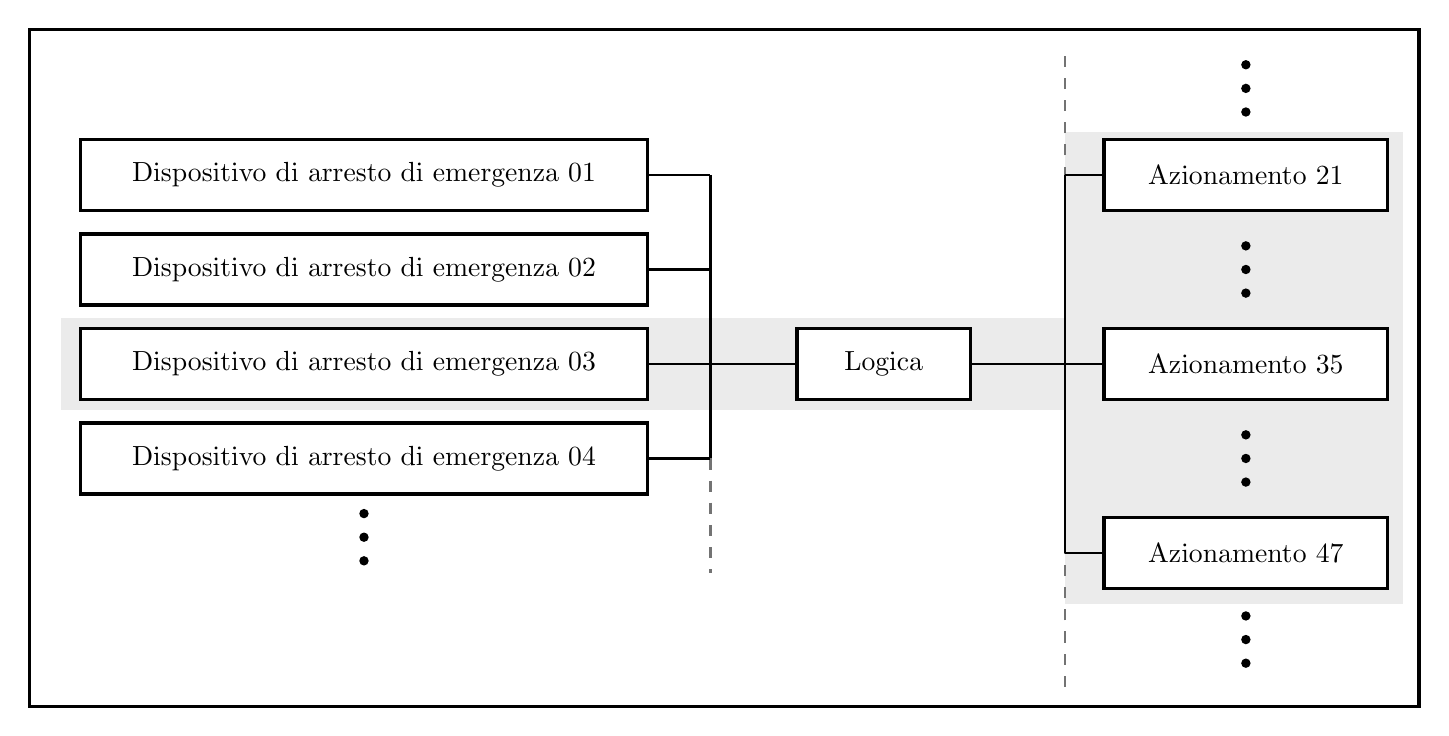
\begin{tikzpicture}[
  font=\normalsize,
  blocco/.style={draw=black, line width=1.2pt, fill=white, align=center,
                 inner sep=4pt, minimum height=0.9cm},
  dispositivo/.style={blocco, minimum width=7.2cm},
  azionamento/.style={blocco, minimum width=3.6cm},
  collegamento/.style={draw=black, line width=0.8pt},
  continua/.style={draw=black!55, line width=0.9pt, dash pattern=on 4pt off 4pt}
]

% Coordinate della cornice, fissate esplicitamente: le linee tratteggiate
% di continuazione devono poter arrivare fin quasi al bordo senza che il
% bordo, ricavato dal bounding box, le insegua.
\def\cornicesx{-0.55}
\def\cornicedx{17.10}
\def\cornicegiu{-0.75}
\def\cornicesu{7.85}

% ---- campiture: cio' che rientra nel caso peggiore -----------------
\fill[black!8] (-0.15,3.02) rectangle (16.90,4.18);   % fascia orizzontale
\fill[black!8] (12.60,0.55) rectangle (16.90,6.55);   % colonna azionamenti

% ---- blocchi: dispositivi di arresto di emergenza ------------------
\node[dispositivo] (d1) at (3.7,6.0) {Dispositivo di arresto di emergenza 01};
\node[dispositivo] (d2) at (3.7,4.8) {Dispositivo di arresto di emergenza 02};
\node[dispositivo] (d3) at (3.7,3.6) {Dispositivo di arresto di emergenza 03};
\node[dispositivo] (d4) at (3.7,2.4) {Dispositivo di arresto di emergenza 04};

\node[blocco, minimum width=2.2cm] (logica) at (10.3,3.6) {Logica};

% ---- blocchi: azionamenti ------------------------------------------
\node[azionamento] (a21) at (14.9,6.0) {Azionamento 21};
\node[azionamento] (a35) at (14.9,3.6) {Azionamento 35};
\node[azionamento] (a47) at (14.9,1.2) {Azionamento 47};

% ---- puntini di continuazione --------------------------------------
\foreach \y in {1.70,1.40,1.10} \fill[black] (3.7,\y) circle (1.7pt);
\foreach \y in {7.40,7.10,6.80} \fill[black] (14.9,\y) circle (1.7pt);
\foreach \y in {5.10,4.80,4.50} \fill[black] (14.9,\y) circle (1.7pt);
\foreach \y in {2.70,2.40,2.10} \fill[black] (14.9,\y) circle (1.7pt);
\foreach \y in {0.40,0.10,-0.20} \fill[black] (14.9,\y) circle (1.7pt);

% ---- collegamenti ---------------------------------------------------
% linea di raccolta dei dispositivi, con proseguimento tratteggiato
\draw[collegamento] (8.1,6.0) -- (8.1,2.4);
\draw[continua]     (8.1,2.4) -- (8.1,0.95);
\draw[collegamento] (d1.east) -- (8.1,6.0);
\draw[collegamento] (d2.east) -- (8.1,4.8);
\draw[collegamento] (d4.east) -- (8.1,2.4);
\draw[collegamento] (d3.east) -- (logica.west);      % dispositivo 03 -> logica

% linea di distribuzione agli azionamenti: tratteggiata per tutta
% l'altezza (gli azionamenti sono cinquanta), continua nel tratto servito
\draw[continua]     (12.6,\cornicegiu+0.25) -- (12.6,\cornicesu-0.25);
\draw[collegamento] (12.6,6.0) -- (12.6,1.2);
\draw[collegamento] (logica.east) -- (a35.west);
\draw[collegamento] (12.6,6.0) -- (a21.west);
\draw[collegamento] (12.6,1.2) -- (a47.west);

% ---- cornice esterna -------------------------------------------------
\draw[draw=black, line width=1.2pt]
  (\cornicesx,\cornicegiu) rectangle (\cornicedx,\cornicesu);

\end{tikzpicture}
